\section{Genetic algorithm (GA) \cite{ai/book/Artificial-Intelligence-A-Modern-Approach/Russell-Norvig}}
\label{AI: Algorithms/Genetic algorithm (GA)}


\begin{figure}[H]
    \centering
    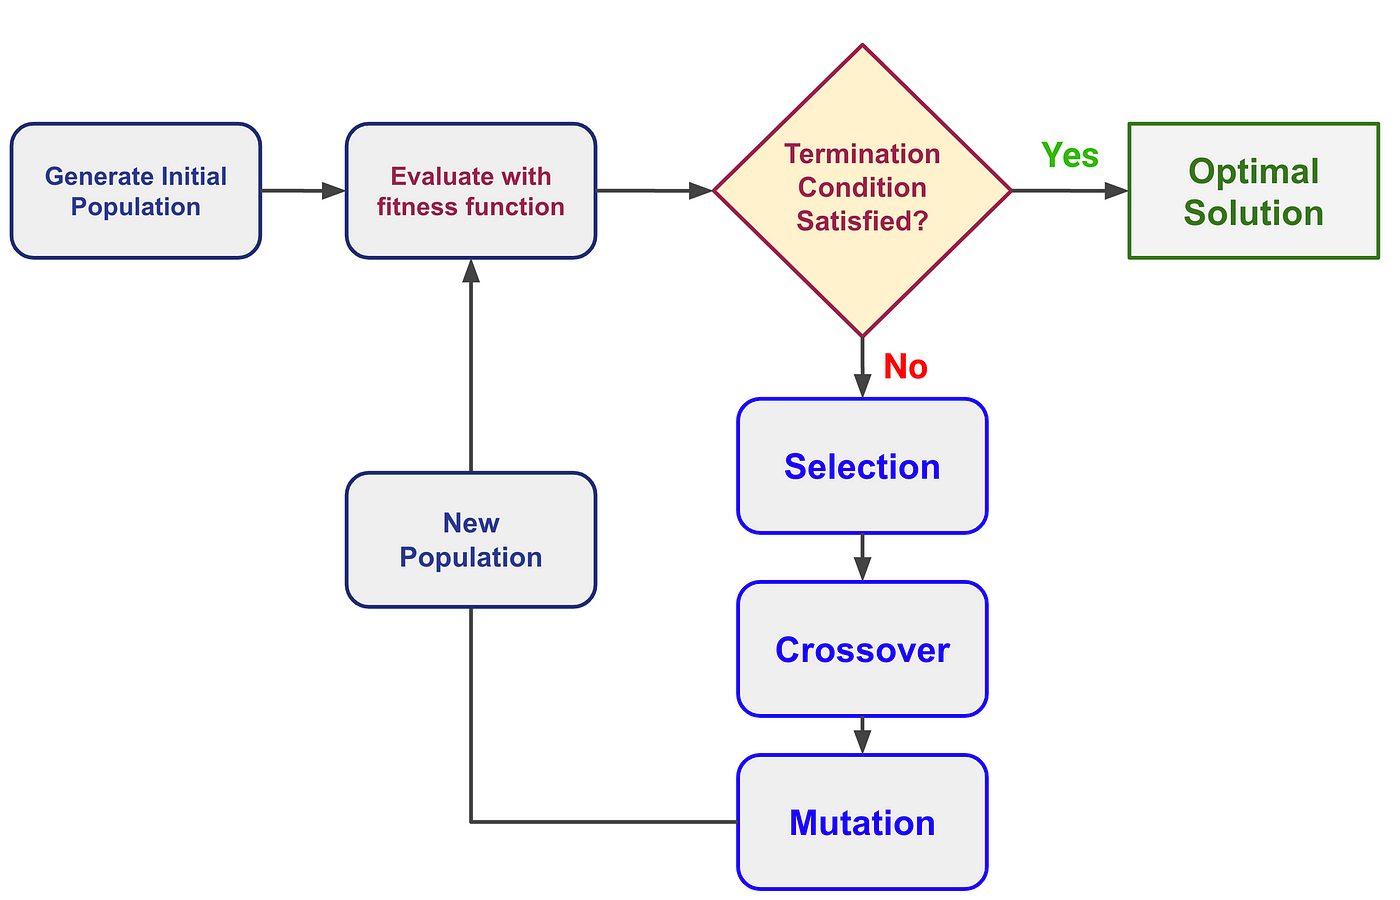
\includegraphics[
        width=\linewidth,
        height=6cm,
        keepaspectratio,
    ]{images/artificial-intelligence/searching/genetic-algorithm-flowchart.png}
    \caption{Genetic Algorithm - flowchart}
\end{figure}


\begin{enumerate}
    \item A genetic algorithm (GA) is a variant of stochastic beam search in which successor states are generated by combining \textit{two} parent states rather than by modifying a single state.
    \hfill \cite{ai/book/Artificial-Intelligence-A-Modern-Approach/Russell-Norvig}

    \item Like beam searches, GAs begin with a set of k randomly generated states, called the population. 
    Each state, or individual, is represented as a string over a finite alphabet—most commonly, a string of $0$s and $1$s.
    \hfill \cite{ai/book/Artificial-Intelligence-A-Modern-Approach/Russell-Norvig}

    \item \textbf{culling}: all individuals below a given threshold are discarded, can be shown to converge faster than the random version
    \hfill \cite{ai/book/Artificial-Intelligence-A-Modern-Approach/Russell-Norvig}

    \item \textbf{steps}:
    \begin{enumerate}
        \item population states
        \hfill \cite{ai/book/Artificial-Intelligence-A-Modern-Approach/Russell-Norvig}

        \item each state is rated by the objective function, or (in GA terminology) the \textbf{fitness function}.
        A fitness function should return higher values for better states
        \hfill \cite{ai/book/Artificial-Intelligence-A-Modern-Approach/Russell-Norvig}

        \item two pairs are selected at \textbf{random} for \textbf{reproduction}, in accordance with the probabilities in (b).
        For each pair to be mated, a \textbf{crossover point} is chosen randomly from the positions in the string.
        \hfill \cite{ai/book/Artificial-Intelligence-A-Modern-Approach/Russell-Norvig}

        \item the offspring themselves are created by crossing over the parent strings at the crossover point.
        When two parent states are quite different, the crossover operation can produce a state that is a long way from either parent state. 
        It is often the case that the population is quite diverse early on in the process, so crossover (like simulated annealing) frequently takes large steps in the state space early in the search process and smaller steps later on when most individuals are quite similar
        \hfill \cite{ai/book/Artificial-Intelligence-A-Modern-Approach/Russell-Norvig}

        \item each location (gene) is subject to random \textbf{mutation} with a small independent probability. 
        \hfill \cite{ai/book/Artificial-Intelligence-A-Modern-Approach/Russell-Norvig}
    \end{enumerate}

    \item Like stochastic beam search, genetic algorithms combine an uphill tendency with random exploration and exchange of information among parallel search threads.
    \hfill \cite{ai/book/Artificial-Intelligence-A-Modern-Approach/Russell-Norvig}

    \item The primary advantage, if any, of genetic algorithms comes from the crossover operation. 
    Yet it can be shown mathematically that, if the positions of the genetic code are permuted initially in a random order, crossover conveys no advantage. 
    \hfill \cite{ai/book/Artificial-Intelligence-A-Modern-Approach/Russell-Norvig}
\end{enumerate}

















